\documentclass[12pt, letterpaper]{article}
\usepackage[utf8]{inputenc}
\usepackage{graphicx}
\usepackage[margin=0.5in]{geometry}
\usepackage{float}
\usepackage{enumitem}
\title{A Support tool for Boolean Networks}
\date{09-06-2021}
\author{Joseph Straw}
\begin{document}
  \pagenumbering{gobble}
  \maketitle
  \newpage
  \pagenumbering{arabic}

  \section{Introduction}

    Boolean networks are a well-studied discrete model used to emulate more
    complex systems. Good examples of their uses are within biological
    networks such as gene regulatory networks \cite{SCHWAB2020571} \cite{TRAN2016107}. 
    The applications are also wider-ranging than just biological systems and may also
    be used to emulate control systems \cite{Valverde:2020we}.

    A Boolean network is constructed from a set of nodes whose state is 
    dictated by a Boolean value. These correspond to 1(active) and 0(inactive). 
    Each node has attached a set of rules dictating what value it should be set 
    to on the next round of iteration, these may be in the form of logical 
    expressions or truth tables. For the example of genes, the nodes would 
    represent those genes and the edges the interactions between them \cite{RISTEVSKI2015111}.

    A consistent problem with boolean networks pertains to the state space explosion.
    This simply describes the exponential complexity of a Boolean network as the 
    number of nodes increases. Due to the nature of each node being able to start from 
    any state, this allows for \(2^n\) number of starting states. As a node is added to 
    the network this will double the number of states availiable. In Figure \ref{fig:BoolNet} C
    it is clear that with a 3 node state that there are 8 permutations for this network. Due 
    to this specific approaches have to be taken. This can include splitting up larger networks 
    or simpler approaches like only processing requested traces \cite{RISTEVSKI2015111}.

    There are also some more minor nuances with the structure and form of the network as detailed in 
    \cite{10.3389/fphys.2018.00586}. For the current application however, synchronus and asynchronus networks
    will be the focus.
    
    \begin{figure}[H]
      \begin{center}
        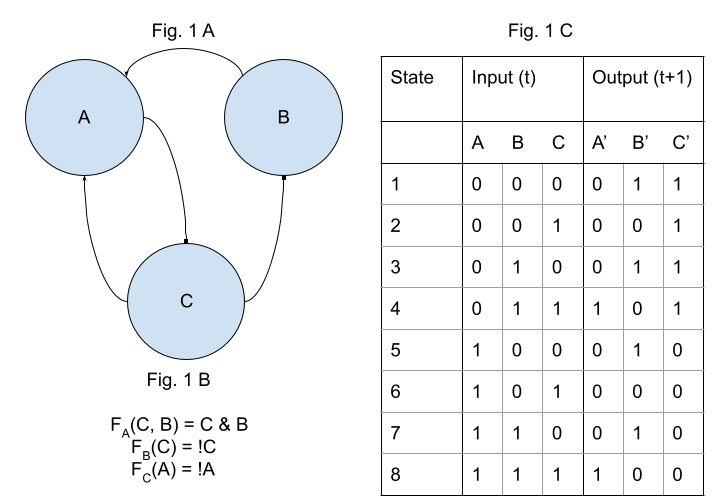
\includegraphics[scale=0.5]{Fig.1.png}
      \end{center}
      \caption{A Boolean network descriptor (A), expressions (B) and truth table (C).}
      \label{fig:BoolNet}
    \end{figure}

    The end goal of this project is the design and develop a Boolean network support tool. It should 
    have the ability to construct, analyse and visualise Boolean networks. There are current tools
    that are availiable that are designed for some or all of these tasks depending on their scope.
    \begin{enumerate}[noitemsep]
      \item Boolesim \cite{Boolesim}
      \item VisiBool \cite{Visibool}
      \item GinSim \cite{Ginsim}
    \end{enumerate}

  \newpage

  \section{Aims and Obejectives}

    The aim of this project is to develop a support tool for Boolean networks, 
    specifically for the case of their construction, analysis and visualisation.

    \subsection{Project objectives:}
    \begin{enumerate}[noitemsep]
      \item Research example boolean networks
      \item Research and evaluate current Boolean network tools
      \item Identify the key requirements for this tool 
      \item Identify user necessities for the tool
      \item Develop approaches to visualise Boolean networks
      \item Research and develop techniques to combat state space explosion
      \item Develop a prototype support tool for Boolean networks
      \item Perform user studies and effectiveness of developed tool (Evaluate the end tool)  
    \end{enumerate}

  \section{Progress}

  \subsection{test}

  \newpage

  \section{Project Plan}

  \begin{figure}[H]
    \begin{center}
      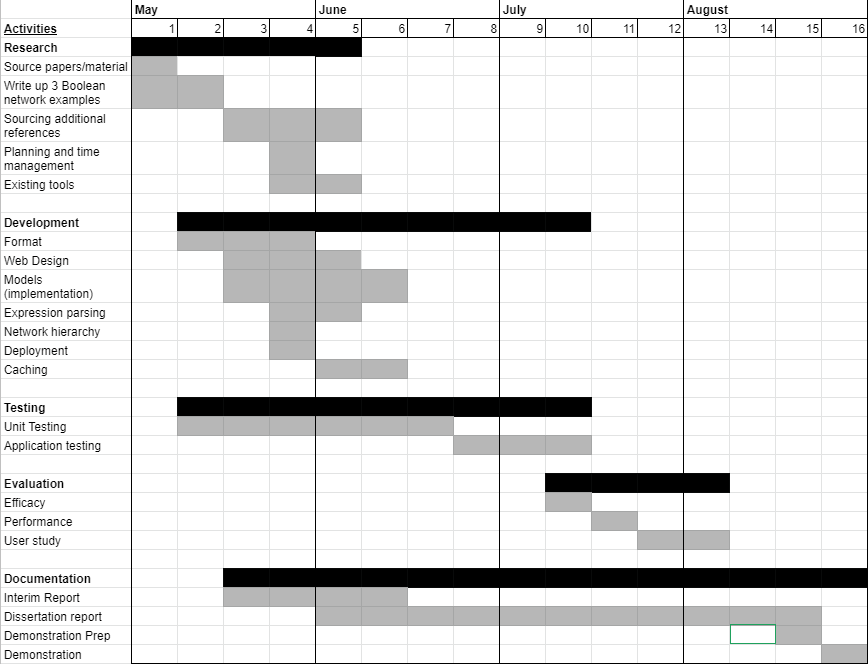
\includegraphics[scale=0.5]{Chart.png}
    \end{center}
    \caption{Project plan gantt chart}
    \label{fig:BoolNet}
  \end{figure}

  \newpage

  \bibliographystyle{IEEEtran}
  \bibliography{InterimReportRefs}
\end{document}